Des données transmissent en utilisant le protocole IPv4 sont encapsulées dans un message que
l'on appelle un paquet IPv4. Ces paquets sont consitué d'un entête suivis des données à transmettre.

% Mossi
\subsection{Adresse IPv4}

L'entête contient des informations essentielles pour la transmission d'un paquet, notamment les
adresses source et destination.

Une adresse IP sert à identifier une machine (et plus précisement une des interfaces de cette machine)
dans un réseau particulié.
Comme nous le verrons plus tard cet identifiant unique permet de désigner à la fois un
réseau et une machine précise au sein de ce réseau.
Une adresse est codé sur 32 bits ce qui permet de coder 2^32 soit 4294967296 adresses différentes.
Par convention on peut représenter une adresse IPv4 comme une suite de 4 nombres décimaux séparés par des points,
chacun traduisant un octet. Cette représentation a contribuée à simplifier l'utilisation et la manipulation
des adresses.
Comme chaque nombre représente un octet, les valeurs de celui-ci sont comprises entre 0 et 255.

\vspace{1cm}
Exemple: adresse à valeur décimale: 212.217.0.1 => correspond sous sa forme
binaire à: 11010100.11011001.00000000.00000001
\vspace{1cm}

\subsubsection{Notion de NET ID et HOST ID}
Une adresse IPv4, en tant qu'inditifiant d'une machine dans un réseau, contient deux informations:
une première partie qui identifie le réseau appellé NET ID (les bits de poids fort), une seconde qui identifie l’hôte appeler host-ID (les bits de poids faible).
Les machines qui se trouvent donc sur le même réseau partage le même NET ID pour leur adresse.

La longueur de ces deux parties est variable: la taille du HOST ID dépend de la taille du NET ID. Pour représenter la longueur de ces différentes parties on a introduit la notion de masque

\subsubsection{Masque de réseau}

Le masque sert à représenter la scission entre le NET ID et le HOST ID.
Il est codé sur 32 bits et adopte la même représentation qu'une adresse IP, à savoir
4 nombres décimaux séparé par des points.
La position des bits à 1 dans le masque corresponde à la position des bits définissant le NET ID dans l'adresse IP.
Pour obtenir les bits du NET ID il suffit de faire un ET logique entre l'adresse et son masque. Tous les autres bits (donc les bits à 0)
feront donc partie du HOST ID.
Les bits à 1 sont contiguës et commencent au bit de poids fort: le nombre de bit à 1 dans le masque, donne
le nombre de bit faisant partie du NET ID en partant du bit de poids fort dans l'adresse.

En conséquence plus le nombre de bit à 1 dans le masque est grand, plus le NET ID sera grand, et plus le HOST ID sera petit, car il restera moins de bit pour définir le HOST ID (la somme des deux devant évidemment faire 32 bits).

\begin{center}
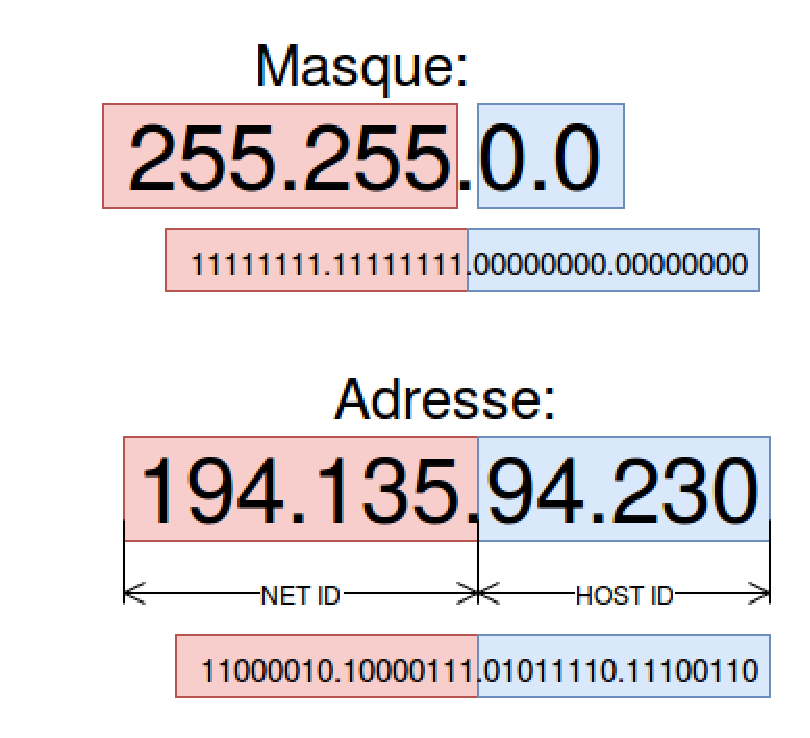
\includegraphics[width=5cm]{./pics/maskipv4.esp}
\end{center}

//TODO exemple
//TODO exemple invalide

\subsubsection{Classes d'adresse IP}



Alors on vient de voir que les adresses IP privées sont utilisable uniquement
sur des réseaux locaux, tandis qu’il y a des adresses IP qui ne sont utilisées
uniquement que sur internet donc nous pouvons en déduir que c’est les adresses
IP publiques non utilisable dans un réseau local. Les routeurs (par exemple:
votre box) ont une adresse IP publique du côté d’internet, ce qui permet de
rendre votre box visible sur internet (elle répondra certainement au ping). De
plus, au moment de vos connexion sur un site web vous utilisez l’adresse
publique du serveur web. De ce fait une adresse IP publique est unique dans le
monde, ce qui n’est pas le cas dans le systèmes d’adressage des adresses IP
privées qui doivent être unique seulement dans un même réseau local mais pas au
niveau planétaire étant donné que ces adresses ne peuvent pas être routées sur
internet. Une adresse IP publique est soit acheté ou fournie par la FAI.  Les
IP publiques représentent toutes les adresses IP des classes A, B et C qui ne
font pas partie de la plage d’adresses privées de ces classes ou des exceptions
de la classe A (voir Adresse non utilisé ci-dessus).


\subsubsection{Les classes d’adresses}
Au début de la création de IPV4, maintes groupes d’adresses ont été définis
pour faciliter le routage (ou cheminement) des paquets. Structurée en 5 classes
(A,B,C,D,E) selon la valeur du première octet.

%TODO images classes %
%TODO tableau recapitulatif %

De ce fait on remarque une distribution de l’espace d’adressage selon laquelle
la classe A possède 50\% l’espace et soit 25\% pour la classe B, 12,5\% classe
C et 6,25\% pour D \& E. on peut en-déduire une mauvaise répartition de cette
espace d’adressage. 

%--------------------------------------
Les classes A, B et C ont chacune une correspondance de plage
d’adresses IP privées à l’intérieur de la plage globale qui a été définie par
la RFC 1918. Mais l’utilisation  de celui-ci pour inter-connecter des réseau
géante (entreprise) avec des espaces adressage qui se chevauche peut causer des
problèmes. Une adresse IP privées est librement paramétrée par l’administrateur
du réseau local.
Les adresses privées de la classe A: 10.0.0.0 à 10.255.255.255\\
Les adresses privées de la classe B: 172.16.0.0 à 172.31.255.255\\
Les adresses privées de la classe C: 192.168.1.0 à 192.168.255.255\\


\textbf{Remarque:}
De ce fait on distingue deux adresses particulières parmi tout ceux possible,
qui ne doivent jamais être attribué à des machines:

     les bits Host-ID sont à 0 : adresse attribue qu’à un réseau.
Exemple: 192.168.10.0 / 255.255.255.0 = 192.168.10.00000000

    les bits Host-ID sont à 1 : c’est un adresse de  diffusion (broadcast),
Exemple: 172.27.255.255 / 255.255.0.0 = 172.27.1111111.11111111

Donc nous pouvons en déduire que parmi tout les adresses assignable, ces
derniers sont des adresses interdites.

\subsubsection{Notation CIDR}
Dans un premier temps nous avons vu que pour connaître l’adresse d’un
réseau il faut forcement passé par le masque, une seconde forme existe et est
connue sous le nom de notation CIDR (classless inter-domain routing) RFC 1519
ou l’adressage sans classe, ce qui veut dire qu’ici on ne tient plus compte de
l’adressage par classe; Donc aucun masque n’est fixé par rapport à une classe.
Elle s’écrit avec le numéro du réseau suivi d’un slash et le nombre de bits à 1
(en partant de la gauche) en binaire du masque sous-réseau. De nos jours cette
notation est la plus utiliser car les différentes classes utiliser sont
devenues  obsolètes.
\vspace{1cm}
Exemple: 186.52.0.0/16
\vspace{1cm}
\textbf{Remarque:}\\
cette notation CIDR ne permet pas la construction des masques réseau à trous,
alors que c’était possible dans la construction de base de IPV4 mais rarement
utilisés car fastidieux la gestion.  IPV6 intègre dés sa conception l’écriture
et l’agrégation maximale des routes introduites par CIDR. 


\subsubsection{Adresses non utilisées}
il existe des adresses non utilisable comme adresse IP pour une machine:\\
les adresses réseaux: qui correspond aux adresses qui ont tous les bits de
leur partie hostid à zéro(0);\\
les adresses de diffusion (broadcast): qui correspond aux adresses qui ont
tous les bits de leur partie hostid à un(1)\\
0.0.0.0: utilise par différentes services (table de routage, DHCP) et possède
souvent une signification particulières. \\
127.X.X.X: désigne l’ordinateur lui-même ou dite adresse de bouclage
(lookback), 127.0.0.1 pour le localhost\\
> à 223.255.255.255: pour le multicast et la recherche.\\


